\documentclass[11pt,twocolumn]{article}
\usepackage[margin=1in]{geometry}
\usepackage{graphicx}
\usepackage{booktabs}
\usepackage{amsmath}
\usepackage{hyperref}
\usepackage{natbib}
\usepackage{xcolor}
\usepackage{multirow}

\title{Simulating Creativity: \\
LLMs as Synthetic Participants in Creativity Research}

\author{
Anonymous Authors\\
\textit{For Review}
}

\date{}

\begin{document}
\raggedbottom

\maketitle

\begin{abstract}
Large language models (LLMs) show promise as ``simulacra''---synthetic participants that could accelerate psychometric research and creativity assessment development. However, it remains unclear whether LLM responses authentically replicate human creativity patterns or merely optimize for surface-level metrics. We compare creativity task responses from three LLM configurations---CRPO (Creative Preference Optimization), Llama 3.1 8B, and Gemini 3 Flash---against human responses ($n \approx 240$) across four established creativity tasks: Alternate Uses (AUT), Scientific Creative Thinking (SCTT), Design Problem-Solving, and Story Writing. Using the Creative Assessment Platform (CAP) for AI-based scoring, we find that while all LLMs exceed human originality scores, CRPO---a model fine-tuned on human creativity preferences---produces distributions closest to human patterns across most metrics. Notably, CRPO matches human effectiveness ratings almost perfectly. These findings suggest that preference-optimized models may serve as more valid simulacra for creativity research than base models, with implications for test development and psychometric validation.
\end{abstract}

\section{Introduction}

Large language models (LLMs) are increasingly proposed as ``simulacra''---synthetic participants capable of accelerating psychometric research by generating human-like responses at scale \citep{dillion2023can}. If validated, such simulacra could transform test development, normative studies, and cross-cultural validation by providing large, cost-effective samples that approximate human response patterns.

Recent work demonstrates the viability of this approach for cognitive tasks. \citet{binz2025centaur} trained Centaur on the Psych-101 dataset, comprising responses from over 60,000 participants across 160 behavioral experiments, achieving human-like performance on held-out tasks. This suggests that models can learn generalizable patterns underlying human cognition when trained on sufficiently diverse behavioral data.

The creativity domain presents a particularly compelling test case, as creative responses exhibit high individual variability and resist simple optimization targets. \citet{ismayilzada2025crpo} introduced Creative Preference Optimization (CRPO), fine-tuning Llama 3.1 on the MuCE dataset of over 200,000 human responses across 30+ creativity assessments. CRPO improved alignment with human creativity preferences while preserving response diversity---a key desideratum for psychometric simulacra.

Yet a fundamental question remains: Do creativity-optimized models produce response \textit{distributions} that match human patterns, or do they merely optimize for surface features that AI-based scorers reward? This distinction is critical for psychometric validity. A model achieving high creativity scores through fundamentally non-human-like responses would be unsuitable for test development, where distributional fidelity---not just mean performance---determines ecological validity.

We investigate this question by comparing CRPO against baseline models (Llama 3.1 8B, Gemini 3 Flash) and human participants across four established creativity tasks. Our analysis focuses on \textit{distributional similarity}---the degree to which model response distributions match human patterns---rather than raw performance metrics.

\section{Methods}

\subsection{Participants and Models}

\textbf{Human sample.} We recruited approximately 240 participants via Prolific. Each participant completed all four creativity tasks, with multiple items per task. To create matched samples for comparison, we randomly selected one response per item per participant, yielding 4,683 matched responses.

\textbf{Model configurations.} We evaluated three LLM configurations:
\begin{itemize}
    \item \textbf{CRPO}: Llama 3.1 8B fine-tuned via Creative Preference Optimization on human creativity responses from the MuCE dataset \citep{ismayilzada2025crpo}
    \item \textbf{Llama 3.1 8B}: Base model without creativity-specific training
    \item \textbf{Gemini 2.0 Flash}: Commercial model from Google DeepMind
\end{itemize}

Each model generated responses for 245 synthetic ``participants'' across all items, mirroring the human study structure. Responses were generated via batched API calls with temperature set to 1.0 to encourage response diversity. Each API call simulated one ``participant'' completing all tasks within a single context window.

\subsection{Creativity Tasks}

We administered four tasks spanning divergent thinking, scientific creativity, design problem-solving, and narrative generation:
\begin{itemize}
    \item \textbf{Alternate Uses Task (AUT)}: Generate creative uses for common objects (5 items: brick, newspaper, shoe, paperclip, blanket)
    \item \textbf{Scientific Creative Thinking Task (SCTT)}: Generate hypotheses and research questions for scientific scenarios (5 items)
    \item \textbf{Design Problem-Solving}: Propose solutions to real-world design challenges (5 items)
    \item \textbf{Story Writing}: Write short creative stories incorporating three specified words (4 prompts)
\end{itemize}

\subsection{Scoring}

Responses were evaluated using the Creative Assessment Platform (CAP), an AI-based scoring system that rates responses on a 0--1 scale. CAP provided \textbf{originality} ratings for AUT, SCTT, and Design tasks, and \textbf{effectiveness} ratings for Design only.

For story responses, we employed two complementary metrics: (1) \textbf{Divergent Semantic Integration} (DSI), measuring average pairwise semantic distance between words in the story, and (2) \textbf{MAoSS} (Model-as-a-Scorer), an LLM-based creativity rating. This dual approach allowed us to examine whether distributional patterns differ across scoring methodologies.

\subsection{Analysis}

Our primary outcome measure was \textbf{distributional similarity} between model and human responses, quantified via:
\begin{itemize}
    \item Two-sample Kolmogorov-Smirnov (KS) tests to assess whether creativity score distributions differ significantly between sources
    \item Semantic centroid similarity, computed by embedding all responses using a sentence transformer, calculating the centroid of human responses for each task, and measuring cosine similarity between each model's response centroid and the human centroid
\end{itemize}

We hypothesized that CRPO, trained on human creativity preferences, would produce distributions most similar to human patterns, reflected in non-significant KS tests and higher semantic similarity to human response centroids.

\section{Results}

\subsection{Sample Characteristics}

Table~\ref{tab:samples} shows the sample sizes for each source-task combination after matching (one response per item per participant).

\begin{table}[h]
\centering
\caption{Sample sizes by source and task}
\label{tab:samples}
\begin{tabular}{lrrrr}
\toprule
Source & AUT & Design & SCTT & Story \\
\midrule
Human & 1,191 & 1,158 & 1,185 & 1,149 \\
CRPO & 1,032 & 1,032 & 1,032 & 1,032 \\
Llama Base & 1,004 & 1,004 & 1,004 & 1,004 \\
Gemini & 980 & 980 & 980 & 980 \\
\bottomrule
\end{tabular}
\end{table}

\subsection{Originality Distributions}

Table~\ref{tab:originality} presents the originality score distributions across CAP-scored tasks. All three LLMs scored significantly higher than humans on originality ($p < .001$ for all KS tests), with Gemini achieving the highest mean scores but also the largest divergence from human distributions. Figure~\ref{fig:distributions} visualizes the distribution overlaps across key metrics.

\begin{table}[h]
\centering
\caption{Originality scores (CAP) by source and task}
\label{tab:originality}
\begin{tabular}{llrrr}
\toprule
Task & Source & $M$ & $SD$ & $d$ \\
\midrule
\multirow{4}{*}{AUT}
& Human & .521 & .085 & --- \\
& \textbf{CRPO} & .564 & .091 & \textbf{--0.49} \\
& Llama Base & .592 & .078 & --0.87 \\
& Gemini & .650 & .076 & --1.59 \\
\midrule
\multirow{4}{*}{SCTT}
& Human & .528 & .125 & --- \\
& \textbf{CRPO} & .617 & .111 & \textbf{--0.75} \\
& Llama Base & .686 & .079 & --1.51 \\
& Gemini & .722 & .130 & --1.53 \\
\midrule
\multirow{4}{*}{Design}
& Human & .471 & .146 & --- \\
& \textbf{CRPO} & .603 & .151 & \textbf{--0.89} \\
& Llama Base & .717 & .105 & --1.94 \\
& Gemini & .758 & .131 & --2.07 \\
\bottomrule
\end{tabular}
\end{table}

CRPO consistently produced the smallest effect sizes relative to humans, indicating distributions most similar to human patterns. Gemini showed the largest divergence ($|d| > 1.5$ across all tasks).

\begin{figure*}[t]
\centering
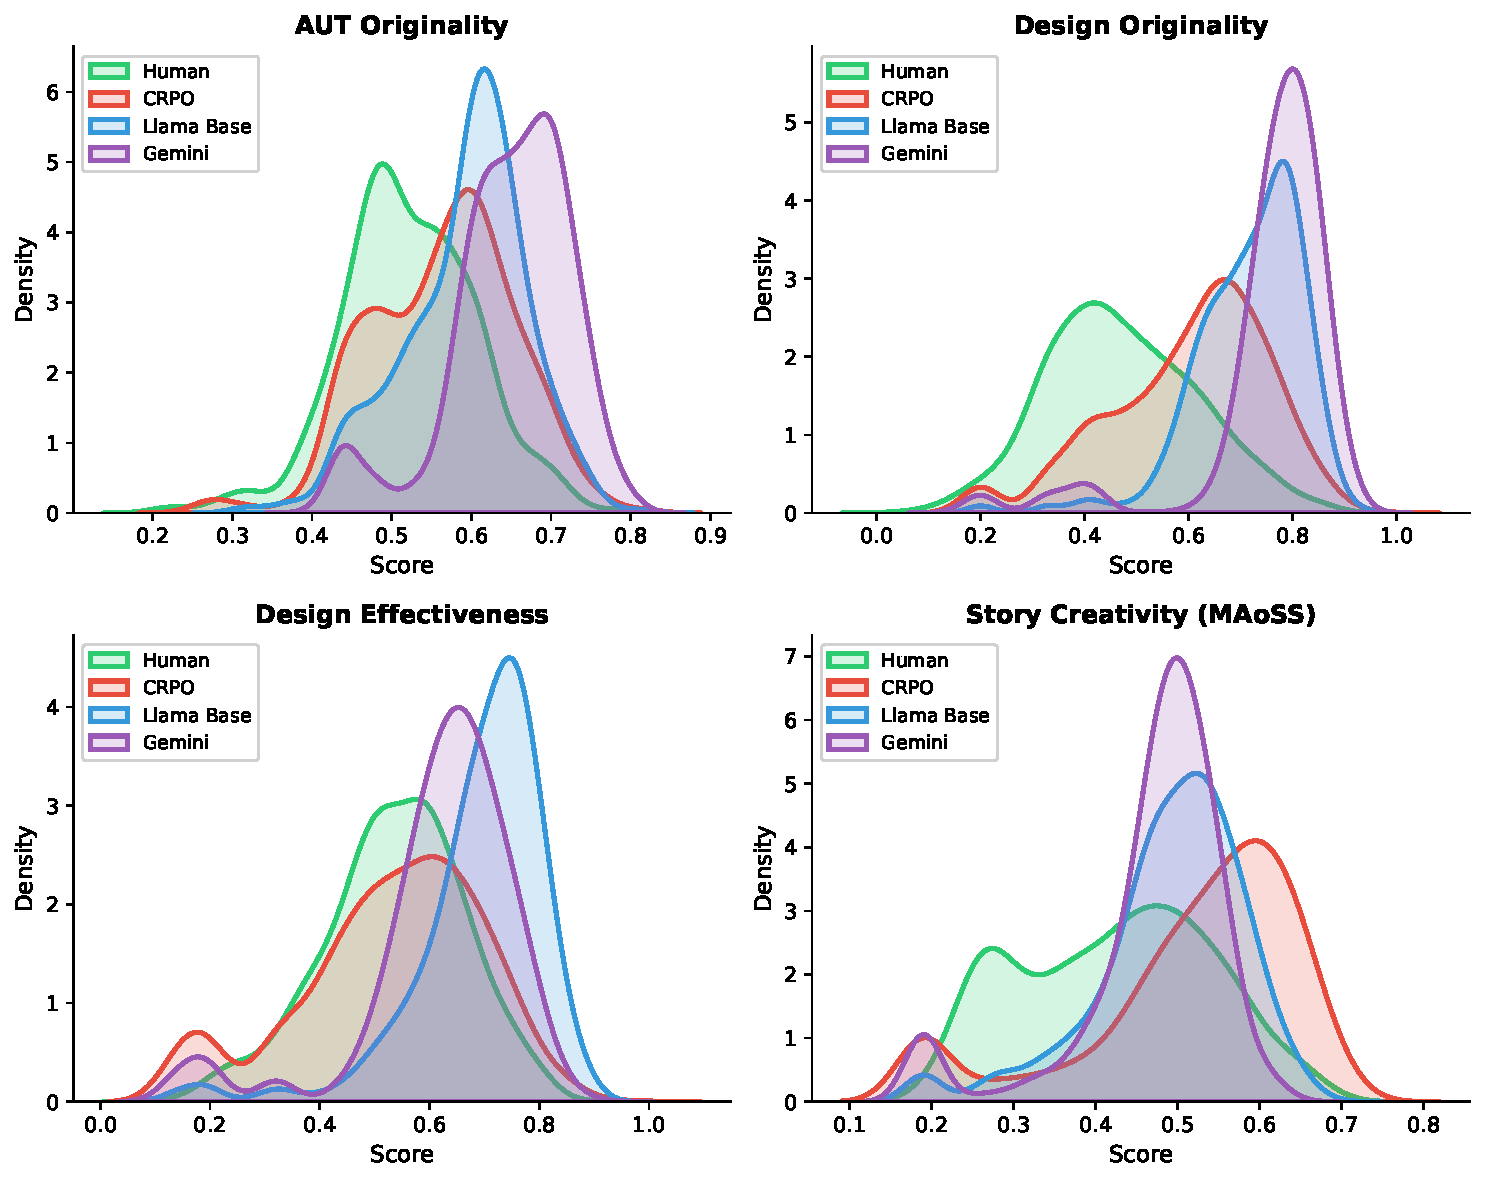
\includegraphics[width=\textwidth]{figures/fig1_distributions.pdf}
\caption{Score distribution overlaps between human and LLM sources across four metrics. CRPO (red) shows the most overlap with human distributions (green) on ideation tasks, while base models diverge substantially. For Design Effectiveness, CRPO nearly perfectly matches the human distribution.}
\label{fig:distributions}
\end{figure*}

\subsection{Design Effectiveness}

A notable exception to the originality pattern emerged for design effectiveness (Table~\ref{tab:effectiveness}). CRPO matched human mean effectiveness almost perfectly ($d = 0.03$, $t$-test $p = .55$), representing the only metric where a model was statistically indistinguishable from humans in central tendency.

\begin{table}[h]
\centering
\caption{Design effectiveness scores (CAP)}
\label{tab:effectiveness}
\begin{tabular}{lrrr}
\toprule
Source & $M$ & $SD$ & $d$ \\
\midrule
Human & .535 & .129 & --- \\
\textbf{CRPO} & \textbf{.532} & .167 & \textbf{0.03} \\
Llama Base & .693 & .121 & --1.26 \\
Gemini & .622 & .139 & --0.65 \\
\bottomrule
\end{tabular}
\end{table}

\subsection{Story Creativity}

Story creativity was assessed using two metrics: DSI (semantic distance) and MAoSS (AI-based rating). These metrics yielded divergent results. For DSI, humans scored higher than all models, with Llama Base closest ($d = 0.20$). For MAoSS (AI-based ratings), LLMs scored higher than humans---consistent with the originality pattern---with Gemini closest to human distributions ($d = -0.45$). This divergence suggests DSI and AI-based ratings capture different aspects of creative writing.

\subsection{Summary: Most Human-Like Model}

Across metrics, CRPO emerged as the most human-like model on 4 of 6 measures, supporting our hypothesis that preference-optimized training produces more valid simulacra. CRPO was closest to human distributions for AUT, SCTT, and Design originality, as well as Design effectiveness. Llama Base was closest on story DSI, and Gemini on story MAoSS. Gemini showed the largest divergence from humans on most metrics.

\section{Discussion}

Our results reveal a nuanced picture of LLM simulacra validity. CRPO produces creativity response distributions most similar to human patterns across ideation tasks, yet all models---including CRPO---systematically exceed human originality scores. This pattern suggests both the promise and limitations of current approaches to psychometric simulation.

\subsection{Training Data and Task Alignment}

CRPO's advantage on ideation tasks (AUT, SCTT, Design) likely reflects task-specific training. The MuCE dataset contains substantial alternate uses and short-form ideation data, providing CRPO direct exposure to human response patterns on these formats. Base models, pretrained predominantly on narrative and expository text, show comparatively better alignment on story writing---a task format closer to their training distribution.

This task-training alignment effect has important implications for simulacra development: domain-specific fine-tuning may be necessary for valid simulation across diverse task types, rather than relying on general-purpose models.

\subsection{The Originality-Effectiveness Dissociation}

A striking dissociation emerged between originality and effectiveness metrics. All models exceeded human originality scores substantially, yet CRPO matched human effectiveness ratings almost perfectly ($d = 0.03$, $p = .55$). This pattern suggests that AI-based originality scoring may inadvertently reward LLM-typical characteristics---unusual word combinations, diverse semantic content, formal register---rather than features characterizing authentic human creativity.

CRPO's preference optimization appears to calibrate responses toward realistic utility judgments while still producing elevated originality scores. This dissociation warrants careful consideration: if AI scorers systematically favor LLM outputs, they may be unsuitable for evaluating simulacra validity without appropriate recalibration.

\subsection{Distributional vs.\ Semantic Similarity}

The story results reveal an instructive dissociation between distributional and semantic measures. CRPO shows the largest divergence from human MAoSS score distributions ($d = -0.72$), yet semantic analysis tells a different story (Figure~\ref{fig:semantic}): CRPO responses exhibit the highest cosine similarity to the human response centroid (0.986 vs.\ 0.969 for Llama Base and 0.972 for Gemini, averaged across tasks).

This apparent contradiction reflects different levels of analysis. CRPO produces stories \textit{semantically} similar to human stories---occupying similar regions of embedding space---but receives different \textit{scores} from the AI rater. The MAoSS model may attend to stylistic or structural features that differentiate CRPO from human outputs, even when semantic content aligns.

\begin{figure*}[t]
\centering
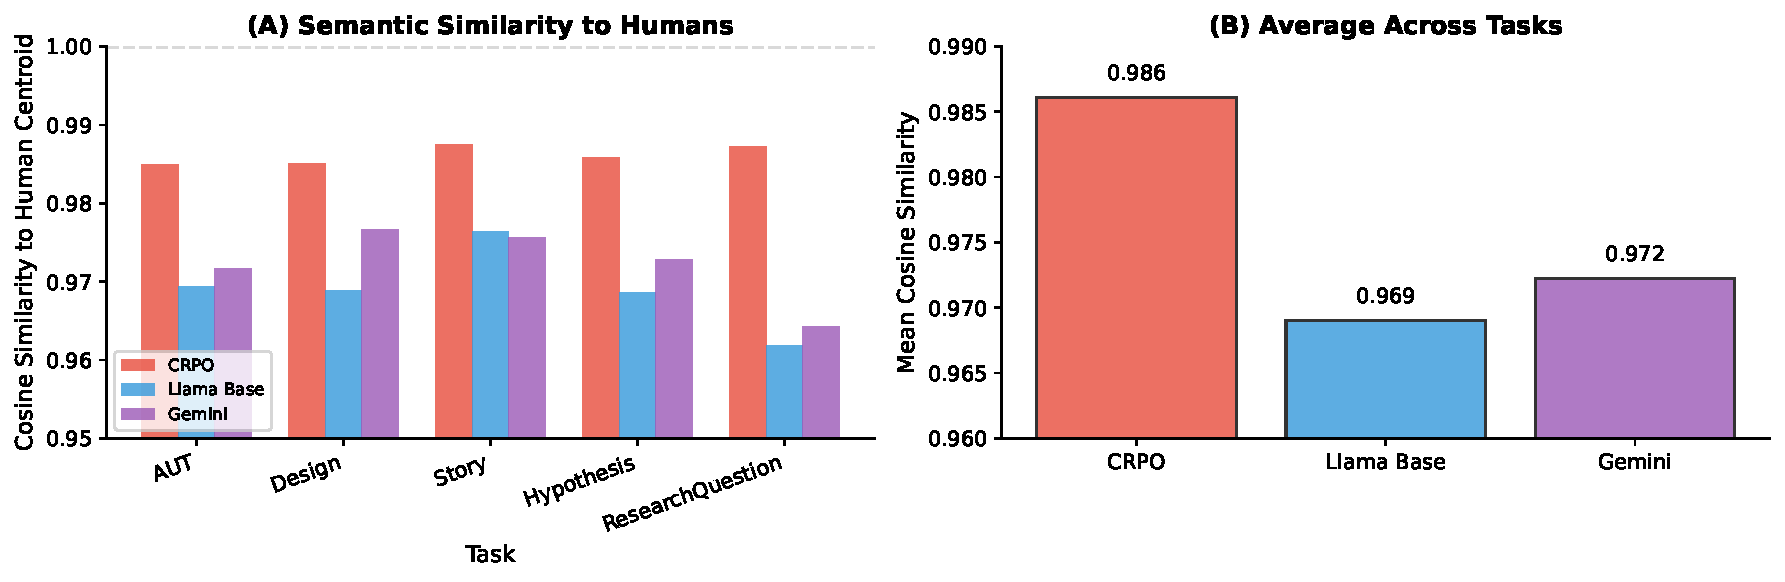
\includegraphics[width=\textwidth]{figures/fig3_semantic_similarity.pdf}
\caption{Semantic similarity to human response centroids. (A) CRPO shows highest similarity across all tasks. (B) Averaged across tasks, CRPO (0.986) exceeds both Llama Base (0.969) and Gemini (0.972), despite showing larger divergence from human creativity \textit{score} distributions.}
\label{fig:semantic}
\end{figure*}

\subsection{Held-Out Generalization}

Notably, only one story prompt (pen-paper-write) appeared in CRPO's training data; the remaining prompts were held out. CRPO's performance across novel prompts suggests some generalization of human-like creativity patterns, though further work is needed to test this hypothesis across additional held-out tasks.

\subsection{Limitations}

Several limitations warrant consideration:

\textbf{Scoring method limitations.} AI-based scoring systems (CAP, MAoSS) may contain systematic biases that differently affect human versus LLM outputs. The consistent pattern of LLMs exceeding human originality scores raises the possibility that these metrics inadvertently reward LLM-typical characteristics (e.g., unusual word combinations, formal language) rather than authentic creativity. The divergence between DSI and MAoSS for story scoring underscores this concern---different metrics yield opposing conclusions about which source is ``more creative.''

\textbf{Training data overlap.} One story prompt (pen-paper-write) appeared in CRPO's training data (MuCE dataset), while other prompts were held out. This limits our ability to fully distinguish learned human-like patterns from memorized responses, though CRPO's consistent performance across held-out prompts suggests some generalization.

\textbf{Prompting strategy.} Baseline models were prompted without specialized techniques. Advanced prompting strategies (e.g., persona prompting, chain-of-thought) may elicit more human-like distributional patterns from base models.

\textbf{Single response sampling.} To match human and LLM sample structures, we randomly selected one response per item per participant. This approach was necessary because LLM responses were generated in batched API calls (one ``participant'' per call, with multiple tasks fit within context), but it limits our ability to examine within-participant response variability.

\textbf{Task scope.} Four creativity tasks, while spanning divergent thinking, problem-solving, and narrative generation, do not capture the full breadth of human creativity (e.g., visual, musical, embodied creativity).

\subsection{Future Directions}

Our findings motivate several extensions:

\begin{enumerate}
    \item \textbf{Novel task generalization}: Testing CRPO on creativity tasks entirely absent from its training data (e.g., metaphor generation) would provide stronger evidence for human-like creativity transfer
    \item \textbf{Cognitive foundation models}: Comparing against Centaur 70B and Minitaur 8B \citep{binz2025centaur} would test whether models trained on broader cognitive data also capture creativity patterns
    \item \textbf{Advanced prompting strategies}: Testing persona prompting, verbalized sampling \citep{zhang2025verbalized}, or other techniques may elicit more human-like distributions from base models
    \item \textbf{Individual differences}: Examining whether LLMs can simulate the full range of human creative ability, including both high and low performers
\end{enumerate}

\section{Conclusion}

CRPO, a model fine-tuned on human creativity preferences, produces creativity score distributions most similar to human patterns across multiple tasks. This suggests that preference-optimized models may serve as more valid simulacra for creativity research than base models, with potential applications in accelerating test development, pilot studies, and psychometric validation. However, the consistent elevation of LLM originality scores relative to humans raises important questions about what AI-based creativity metrics actually measure and whether current scoring systems inadvertently favor LLM-typical outputs.

\bibliographystyle{apalike}
\begin{thebibliography}{9}

\bibitem[Binz et~al., 2025]{binz2025centaur}
Binz, M., Akata, E., Bethge, M., Br\"{a}ndle, F., Callaway, F., Coda-Forno, J., \ldots\ Schulz, E. (2025).
\newblock A foundation model to predict and capture human cognition.
\newblock \emph{Nature}, 644(8078), 1002--1009.

\bibitem[Dillion et~al., 2023]{dillion2023can}
Dillion, D., Tandon, N., Gu, Y., and Gray, K. (2023).
\newblock Can AI language models replace human participants?
\newblock \emph{Trends in Cognitive Sciences}, 27(7), 597--600.

\bibitem[Ismayilzada et~al., 2025]{ismayilzada2025crpo}
Ismayilzada, M., Laverghetta Jr., A., Luchini, S.~A., Patel, R., Beaty, R.~E., Bosselut, A., and van der Plas, L. (2025).
\newblock Creative Preference Optimization.
\newblock In \emph{Findings of the Association for Computational Linguistics: EMNLP 2025}, 9580--9609.

\bibitem[Zhang et~al., 2025]{zhang2025verbalized}
Zhang, J., Yu, S., Chong, D., Sicilia, A., Tomz, M.~R., Manning, C.~D., and Shi, W. (2025).
\newblock Verbalized Sampling: How to Mitigate Mode Collapse and Unlock LLM Diversity.
\newblock \emph{arXiv preprint arXiv:2510.01171}.

\end{thebibliography}

\end{document}
